\documentclass[a4paper, 12pt]{article}
\usepackage[utf8]{inputenc}
\usepackage[german]{babel}
\usepackage[T1]{fontenc}
\usepackage[table]{xcolor}
\usepackage[mathletters]{ucs}
\usepackage{graphicx} 
\usepackage{amsmath}
\usepackage{booktabs,multirow,bigstrut}
\usepackage{hyperref}
\usepackage{cite}
\usepackage{natbib}
\usepackage{url}
\usepackage{diagbox}
\usepackage{enumitem}
\usepackage{tabularx}
\usepackage{tcolorbox}
\usepackage{verbatim}
\usepackage{caption}
\usepackage{float}


%\usepackage[figurename=Fig.]{caption}
%\usepackage[tablename=Tab.]{caption}
%\renewcommand{\thesubsubsection}{\Alph{subsubsection}}
\renewcommand{\thesubsubsection}{\Roman{subsubsection}}

\title{Belegarbeit \\
		- Semesterprojekt - Neuronale Netze -}
\author{Mikroprozessortechnik (CE23) \\
Luca Alexander Schulz\\
Marcus Worrmann\\
HTW Berlin
} 

\date{\today}


\begin{document}
	
\maketitle	

\begin{figure}[h]
	\centering
	
\includegraphics[width=10cm]{Bilders/htw.png}
\end{figure}

\newpage 
\tableofcontents

\newpage %PAGEBREAK

\listoffigures
\listoftables

\newpage %PAGEBREAK

\section{Einleitung}\label{chapter..1}
In der vorliegenden Seminararbeit wird der Entwicklungsprozess eines künstlichen neuronalen Netzes 
detailliert beschrieben. Ziel der Arbeit war die Erkennung von Ziffern, Buchstaben oder Objekten, wobei 
der Schwerpunkt auf der Erkennung von Ziffern mithilfe des MNIST-Datensatzes \cite{MNIST-Datensatz} liegt. 
Die algorithmische Implementierung erfolgt dabei in der Programmiersprache \texttt{C}.\\
Für die unterschiedlichen Varianten des maschinellen Lernens werden Ansätze des sequentiellen 
Lernens als induktiver Algorithmus sowie parallele und SIMD-basierte Methoden zur Erhöhung der 
Parallelität verwendet. Um die Leistungsfähigkeit der verschiedenen Algorithmen zu analysieren, 
werden die Trainingszeiten verglichen, ausgewertet und abschließend diskutiert.\\
Zur tiefergehenden Untersuchung der Qualität der Implementierungen werden darüber hinaus Tools 
wie \texttt{Valgrind} und \texttt{Helgrind} eingesetzt. Diese ermöglichen eine umfassende Analyse 
der Speicherverwaltung und Parallelitätsaspekte.\\
Im weiteren Verlauf wird zunächst die zugrunde liegende Theorie erläutert, gefolgt von einer 
detaillierten Beschreibung der Implementierung der Skripte. Anschließend werden die Ergebnisse 
visualisiert und diskutiert.\\
Abschließend bietet die Arbeit eine Zusammenfassung des Projekts, inklusive der gesteckten und 
erreichten Ziele, sowie einen Ausblick auf mögliche zukünftige Weiterentwicklungen. Ein Fazit 
rundet die Arbeit ab.

\newpage %PAGEBREAK

\section{Theoretische Grundlage}\label{chapter..2}
In diesem Abschnitt werden die historischen Wurzeln, die theoretischen Grundlagen künstlicher 
neuronaler Netze umfassend erläutert. Dabei wird sowohl auf die grundlegenden Konzepte als auch 
auf die mathematischen Prinzipien eingegangen, die der Funktionsweise und dem Training dieser 
Netzwerke zugrunde liegen. Die einzelnen Aspekte werden systematisch dargestellt und eingehend 
analysiert.

\subsection{Historischer Kontext}\label{chapter..2.1}
Die ersten wissenschaftlichen Ansätze zur Erforschung computergestützter Algorithmen, die auf der 
aus der Biologie bekannten Funktionsweise und Verarbeitung von Eindrücken und Informationen in 
neuronalen Netzen basieren, stammen aus den 1950er und 1960er Jahren. Der Psychologe Frank 
Rosenblatt entwickelte das Perzeptron, ein einfaches neuronales Netz, das grundlegende Muster 
erkennen konnte. Mit dem \textit{Mark I Perceptron} war es möglich, Ziffern auf einem 
\texttt{20x20}-Pixel-Sensor zu erkennen. Aufgrund seiner Unfähigkeit, nichtlinear separierbare 
Probleme zu lösen, verlor dieses Modell jedoch an Bedeutung.\cite{kriesel2007kleiner}\\
In den 1980er Jahren erlebten neuronale Netze eine Renaissance durch die Einführung des 
Backpropagation-Algorithmus, beschrieben im Werk \textit{"Backpropagation of Error"}, der eine 
Fehlerkorrektur während des Trainings ermöglichte. Dieser Fortschritt erlaubte es neuronalen Netzen, 
komplexe, nichtlineare Probleme zu lösen und legte den Grundstein für viele moderne Anwendungen der 
künstlichen Intelligenz.\cite{kriesel2007kleiner}\\
Durch die 2015 veröffentlichte Arbeit von Yann LeCun, Yoshua Bengio und Geoffrey Hinton wurde die 
Entwicklung des modernen Deep Learning maßgeblich vorangetrieben.\cite{lecun2015deep} Sie 
kombinierten klassische Konzepte neuronaler Netze mit den heutigen Möglichkeiten leistungsfähiger 
Rechenkapazitäten, großer Datenmengen und verbesserter Netzwerkarchitekturen. Diese Ansätze 
ermöglichten den Durchbruch mehrschichtiger, tiefer neuronaler Netze, die in zahlreichen Bereichen 
wie der Bilderkennung und Sprachverarbeitung bahnbrechende Fortschritte erzielten. Für ihre 
Pionierarbeit erhielten die Forscher 2018 den renommierten Turing Award.

\newpage %PAGEBREAK

\subsection{Grundlagen neuronaler Netze}\label{chapter..2.2}
Die im Verlauf des letzten Jahrhunderts verfolgten Ansätze zielten auf die Entwicklung und 
Implementierung künstlicher neuronaler Netzwerke (KNN) ab, die als leistungsfähige 
Datenverarbeitungsprogramme dienen und in ihrer Funktionsweise biologischen neuronalen Netzwerken 
ähneln \cite{rey2019neuronale}.\\
Der Anwendungsbereich dieser Methoden lässt sich heutzutage in zwei wesentliche Kategorien 
unterteilen:\\

\begin{itemize}
	\item Modellierte KNN zur Simulation und Erforschung der Funktionsweise des menschlichen 
			Gehirns.
    \item KNN zur Lösung spezifischer Anwendungsprobleme in den Bereichen Statistik, Wirtschaft 
			und Technik.
\end{itemize}

In diesem Zusammenhang erweitern künstliche neuronale Netzwerke unsere mathematischen Modelle der 
menschlichen Denkprozesse.\\
Der Aufbau eines solchen Netzwerks ist in der nachfolgenden \autoref{fig:KNN} dargestellt.

\begin{figure}[h]
	\begin{center}
		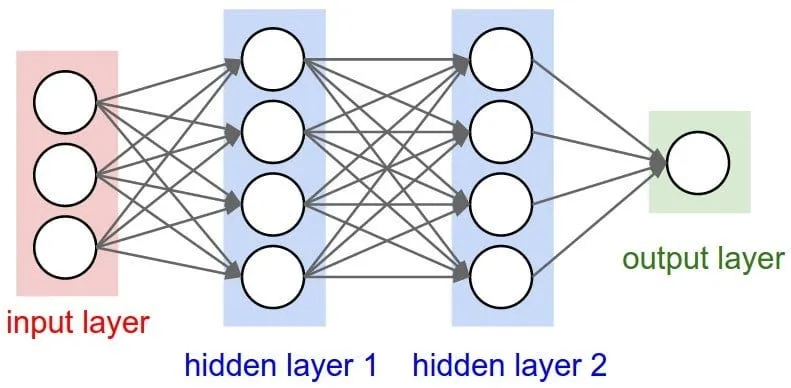
\includegraphics[width=10cm]{Bilders/KNN.png}
		\caption{Schematische Darstellung eines KNN\cite{rahman2023}}
		\label{fig:KNN}
	\end{center}
\end{figure}

Wie in \autoref{fig:KNN} dargestellt, bestehen neuronale Netze aus mehreren Knoten - den sogenannten 
Neuronen - welche auch als Units oder Einheiten bezeichnet werden können. Die Hauptfunktion der 
Neuronen besteht darin, Informationen entweder aus der Umgebung oder von anderen Neuronen zu 
empfangen, diese zu modifizieren und an die Außenwelt oder wiederum an andere Neuronen 
weiterzuleiten. Dabei lassen sich die Neuronen in drei Schichten unterteilen:

\begin{itemize}
    \item \textcolor{red}{\textbf{Input-Layer}}: 
    Der Input-Layer besteht aus Units, die in der Lage sind, externe Signale unterschiedlicher Art 
	zu empfangen. Die Anzahl dieser Units entspricht der Anzahl der Merkmale in den Eingangsdaten.
    
    \item \textcolor{blue}{\textbf{Hidden-Layer}}: 
    Die Hidden-Layer bilden die Schicht von Neuronen, die sich zwischen dem Input- und dem 
	Output-Layer befinden. In diesen Schichten werden die Eingangsdaten weiterverarbeitet, wodurch 
	die Komplexität und Leistungsfähigkeit des Netzwerks maßgeblich beeinflusst wird.
    
    \item \textcolor{green}{\textbf{Output-Layer}}: 
    Der Output-Layer ist die letzte Schicht des Netzwerks und besteht aus Neuronen, die für die 
	Ausgabe des endgültigen Signals an die Außenwelt verantwortlich sind. Die Anzahl der Neuronen 
	in dieser Schicht repräsentiert die Anzahl der Ausgabesignale.
\end{itemize}

Die Units der einzelnen Layer sind durch Kanten miteinander verbunden, deren Verbindungsstärken durch 
Gewichte zwischen den Neuronen definiert werden. Diese Gewichte repräsentieren den Einfluss, den ein 
Signalwert auf das nachfolgende Neuron ausübt, und bestimmen somit die Verstärkung oder Abschwächung 
des Signals.\\
Das Lernverhalten eines neuronalen Netzwerks wird als Anpassung der Gewichte zwischen den Neuronen 
beschrieben.\cite{rey2019neuronale} Die Veränderung dieser Gewichte unterliegt den zugrunde liegenden 
Lernregeln. Diese Lernregeln beruhen häufig auf der Anwendung nichtlinearer Aktivierungsfunktionen, 
die auf die Summe der gewichteten Eingangssignale angewendet werden.\\
Zusammenfassend lassen sich die fundamentalen Bestandteile und Strukturen eines neuronalen Netzwerks 
wie folgt beschreiben:

\begin{itemize}
	\item \textbf{Neuron}: Ein Neuron empfängt eine ein oder mehrere Eingangssignale, welche jeweils mit 
						   zugehörigen Gewichten multipliziert werden. Anschließend werden die 
						   gewichteten Eingangssignale summiert, und das Ergebnis wird durch eine 
						   Aktivierungsfunktion verarbeitet. Das Ergebnis dieser Aktivierungsfunktion 
						   bestimmt, ob und in welcher Intensität das Neuron ein Ausgangssignal an 
						   nachfolgende Neuronen weitergibt.
	\item \textbf{Gewichte}: Die Verbindungen zwischen Neuronen werden durch Gewichte charakterisiert, 
							 die den Einfluss eines Eingangssignals auf das nachfolgende Neuron 
							 bestimmen. Diese Gewichte werden während des Trainingsprozesses 
							 kontinuierlich angepasst, um die Leistung des Modells zu optimieren. 
							 Der Trainingsprozess zielt darauf ab, die Gewichte so zu modifizieren, 
							 Abweichungen zwischen den Vorhersagen des Modells und den tatsächlichen 
							 Ausgaben minimiert werden. Die Gewichte lassen sich basierend auf ihrem 
							 Einfluss auf die Signalübertragung in drei Kategorien einteilen:
			\begin{enumerate}[label=\textbf{[\Alph*]}]
				\item \textit{Positives Gewicht}: Ein Neuron übt einen exzitatorischen, also stimulierenden Einfluss auf ein anderes Neuron aus.
				\item \textit{Negatives Gewicht}: Ein Neuron übt einen inhibitorischen, also hemmenden Einfluss auf ein anderes Neuron aus.
				\item \textit{Gewicht von Null}: Ein Neuron hat keinen Einfluss auf ein jeweils anderes Neuron.
			\end{enumerate}
							
    \item \textbf{Schichten}: Die verschiedenen Schichten eines neuronalen Netzwerks dienen als 
							  spezialisierte Einheiten, die unterschiedliche Aufgaben der 
							  Datenverarbeitung und Mustererkennung übernehmen.    
	\item \textbf{Aktivierungsfunktion}: Aktivierungsfunktionen, auch als Transferfunktionen bezeichnet, 
					bestimmen die Beziehung zwischen dem Netzinput und dem Aktivitätsniveau eines 
					Neurons. Sie spielen eine zentrale Rolle in neuronalen Netzwerken, in der Umsetzung der
					nichtlinearität eines Modells, welche notwendig ist, um komplexe Muster zu 
					lernen und darzustellen. Zu den wichtigsten Aktivierungsfunktionen gehören hierbei die 
					\texttt{Sigmoid}-Funktion, der \texttt{Hyperbolische Tangens (Tanh)} sowie die 
					\texttt{ReLU}-Funktion (Rectified Linear Unit). Durch diese Funktionen besitzt ein
					neuronales Netzwerk die Fähigkeit, differenzierte Zusammenhänge im Datenraum zu 
					modellieren.

\end{itemize}

\newpage %PAGEBREAK

\subsection{Mathematische Herleitung}\label{chapter..2.3}

Grundsätzlich lassen sich neuronale Netze kompakt in Form von Matrizen darstellen. Eine solche Matrix, 
bezeichnet als \( W \), besteht aus einer Menge von Elementen \( w_{ij} \), wobei \( i \) die 
Output-Unit und \( j \) die Input-Unit repräsentiert. Da das Lernen in neuronalen Netzen auf der 
Anpassung von Gewichten basiert, werden diese Netzgewichte durch die Matrix abgebildet. Einfache 
neuronale Netze, die keine Hidden-Layers beinhalten, können durch eine einzelne 
Matrix dargestellt werden. Für neuronale Netze mit Hidden-Layern wird für jede dieser Schichten 
eine separate Gewichtsmatrix benötigt, um die entsprechenden Verbindungen darzustellen.\\
Die Struktur einer solchen Matrix für ein einfaches neuronales Netz ohne Hidden-Layer kann 
folgendermaßen aussehen:

\[
W = 
\begin{bmatrix}
w_{11} & w_{12} & w_{13} & w_{14} \\
w_{21} & w_{22} & w_{23} & w_{24} \\
w_{31} & w_{32} & w_{33} & w_{34}
\end{bmatrix}
\]

Diese mathematische Darstellung ist jedoch nicht ausreichend für neuronale Netze, die in der Lage sein 
sollen, komplexe und differenzierte Zusammenhänge zu modellieren, wie sie die in \autoref{chapter..2.2} 
genannten Aktivierungsfunktionen erfordern. Um die Transformationen solcher Funktionen zu modellieren, 
kann folgende mathematische Grundlage verwendet werden, bei der ein einzelnes Neuron sein 
Ausgangssignal \( y \) wie folgt berechnet:

\[
y = f\left( \sum w_i * x_i + b \right)
\]

\begin{table}[ht]
    \centering
    \begin{tabular}{|c|l|}
        \hline
        \textbf{Symbol} & \textbf{Beschreibung} \\
        \hline
        \(y\) & Ausgangssignal des Neurons \\
        \(f\) & Aktivierungsfunktion (z.B. Sigmoid, Tanh, ReLU) \\
        \(\sum\) & Summe der gewichteten Eingaben \\
        \(w_i\) & Gewicht für den \(i\)-ten Eingabewert \\
        \(x_i\) & Eingabewert zum Neuron \\
        \(b\) & Bias (Verschiebungsterm) \\
        \hline
    \end{tabular}
	\caption{Parameter der Neuronen-Gleichung}
    \label{tab:neuron_para}
\end{table}

Wie in \autoref{tab:neuron_para} dargestellt, können Aktivierungsfunktionen hinsichtlich ihrer Form 
unterschieden werden. Sie lassen sich nach dem zugrunde liegenden Netzinput und dem gewünschten 
Aktivitätsniveau klassifizieren. Die nachfolgende Tabelle bietet einen kurzen Überblick über 
verschiedene Aktivierungsfunktionen und ihre Eigenschaften:

\begin{table}[h!]
	\centering
	\begin{tabular}{|>{\centering\arraybackslash}m{2.8cm}|>{\raggedright\arraybackslash}m{6.5cm}|>{\centering\arraybackslash}m{2.8cm}|}
	\hline
	\textbf{Funktionsart} & \textbf{Funktion} & \textbf{Formel} \\ \hline
	{Sigmoid} & Transformiert Eingaben in einen Bereich zwischen 0 und 1. Häufiger Einsatz für binäre Entscheidungen. Ähnlich der binären Schwellenfunktion. & \(f(x) = \frac{1}{1 + e^{-x}}\) \\ \hline
	{Hyperbolischer Tangens} & \vspace{0.2cm}Transformiert Eingaben in einen Bereich zwischen -1 und 1. Nützlich für zentrierte Ausgaben.\vspace{0.2cm} & \(f(x) = \tanh(x)\) \\ \hline
	{ReLU} & \vspace{0.2cm}Setzt negative Werte auf Null und behält positive Werte bei.\vspace{0.2cm} & \(f(x) = \max(0, x)\) \\ \hline
	\end{tabular}
	\caption{Arten von Aktivierungsfunktionen}
	\label{tab:Aktivierungsfunktion}
\end{table}

Ein wesentliches Problem, das bei der Verwendung von Netzen mit Hidden-Layers auftritt, ist die 
mangelnde Transparenz des Fehlerpotenzials der Neuronen in diesen Schichten. Im Gegensatz zu 
einfachen Netzen, bei denen der Fehlerausdruck im Output direkt erkennbar ist, muss dieser Fehlerterm 
in komplexeren Systemen auf andere Weise ermittelt werden. Die Anpassung der Gewichte erfolgt im 
Laufe verschiedener Trainingsphasen, wobei die Gewichtsänderung in drei Schritten vollzogen wird.

\subsubsection{Forward Propagation}\label{chapter..2.3.1}
Die Inferenz, auch als \textit{Forward Propagation} bekannt, beschreibt den Prozess, bei dem der 
Input durch die Neuronen im Netzwerk weitergeleitet wird, um bestimmte Outputs zu berechnen. Jede 
Schicht erhält dabei schrittweise den Ausgabewert der vorherigen Schicht als Eingabe, bis das 
Netzwerk komplett durchlaufen wurde und ein Output am Output-Layer berechnet werden kann. 
Mathematisch lässt sich dieser Prozess durch die folgende Gleichung darstellen, wobei $l_i$ den 
Output der $i$-ten Schicht darstellt:

\[
l_{i+1} = f(w_i \cdot l_i + b_i)
\]

\newpage %PAGEBREAK

\subsubsection{Fehlerbestimmung}\label{chapter..2.3.2}
Im zweiten Schritt, der Fehlerbestimmung, wird die Differenz zwischen dem gewünschten Ausgabewert 
$y_\text{true}$ und dem durch die Forward Propagation tatsächlich erzielten Ausgabewert 
$y_\text{pred}$ ermittelt. Dieser Fehler $E$ wird durch die nachfolgende quadratische Fehlerfunktion 
berechnet. Der Vorteil einer quadratischen Mittelwertbestimmung liegt darin, dass ausschließlich 
positive Ergebnisse erzielt werden, was die Aufsummierung erleichtert. Zudem fallen große Fehler 
stärker ins Gewicht, was für den dritten Schritt im Lernprozess ausschlaggebend ist.

\[
E = \frac{1}{2} (y_\text{true} - y_\text{pred})^2
\]

\subsubsection{Back Propagation}\label{chapter..2.3.3}
Überschreiten die in \autoref{chapter..2.3.2} genannten Fehler einen definierten Gütewert, so werden 
im finalen Schritt die Gewichte der Hidden-Layer angepasst. Hierfür werden die Fehlerterme 
entgegengesetzt rückwirkend zum Input-Layer angepasst. Das bedeutet, dass zunächst die Gewichte 
zwischen dem Output-Layer und dem letzten Hidden-Layer modifiziert werden und sich sukzessiv zum 
Input-Layer vorgearbeitet wird. Die Gewichte werden nach folgender Gleichung angepasst, um die 
Fehlerterme zu verringern. Für jedes Gewicht $w$ wird das Update über die Lernrate $\eta$ und 
$\frac{\partial E}{\partial w}$ als Gradient des Fehlers vom anfänglichen Gewicht abgezogen:

\[
w_\text{neu} = w_\text{alt} - \eta \cdot \frac{\partial E}{\partial w}
\]

Es sei erwähnt, dass es durchaus noch weitere Lernregeln und Methodiken wie die \textit{Hebb-Regel}, 
die \textit{Delta-Regel} oder das \textit{Competitive-Learning} gibt. Da in dieser Arbeit jedoch 
die Methoden der Backpropagation im Fokus stehen, werden die anderen Regeln nicht weiter beleuchtet.

\newpage %PAGEBREAK

\section{Implementierung des neuronalen Netzwerks}\label{chapter..3}

In diesem Kapitel wird die Herangehensweise zur Umsetzung und Implementierung des Codes eines 
neuronalen Netzes beschrieben. Der Schwerpunkt liegt auf dem zugrunde liegenden MNIST-Datensatz, 
der als Trainingsgrundlage dient. Zudem werden die einzelnen Strukturen innerhalb des Codes, die 
in \autoref{chapter..2} erläutert wurden, sowie verschiedene Ansätze zur Optimierung der 
Algorithmen und des implementierten Codes detailliert betrachtet.

\subsection{MNIST-Datensatz}\label{chapter..3.1}

Der MNIST-Datensatz (Modified National Institute of Standards and Technology) gilt als einer der 
bekanntesten Datensätze im Bereich des maschinellen Lernens. Zudem wird er häufig als Test- und 
Trainingsgrundlage für Bildklassifikationsalgorithmen verwendet. Der Datensatz wurde über 
\textit{TensorFlow} heruntergeladen und umfasst folgende zwei separate CSV-Dateien:

\begin{center}
	\texttt{train-images.idx3-ubyte}
\end{center}

\begin{center}
	\texttt{train-labels.idx1-ubyte}
\end{center}

Insgesamt enthält der Datensatz 70.000 Bilder handgeschriebener Ziffern im Bereich von 0 bis 9. 
Für Trainingszwecke werden 60.000 der Bilder verwendet, während die restlichen 10.000 zur 
Validierung und zur Berechnung der Genauigkeit herangezogen werden.

\subsection{Lernmethoden} 
\subsubsection{Forward Propagation} 
\subsubsection{Fehlerbestimmung} 
\subsubsection{Backpropagation}

\subsection{Berechnung der Genauigkeit}

\subsection{Implementierungsansätze} 
\subsubsection{Sequentiell} 
\subsubsection{Parallel} 
\subsubsection{SIMD}

\newpage %PAGEBREAK

\section{Ergebnisse}\label{chapter..4}

In diesem Abschnitt werden die Ergebnisse, welche aus diskreten Parametern erzielt wurden, näher 
beschrieben und anhand visueller Ausgaben durch das Plottool \textit{R} vorgestellt. Dabei wird der 
Seed zur Erzeugung der Daten detailliert beschrieben sowie die durch Tools wie \textit{Hyperfine} 
ermittelten Benchmarks genutzt. Die Ergebnisse der unterschiedlichen Algorithmen sowie das zur 
Ermittlung der Daten genutzte System können der \autoref{fig:plot} entnommen werden.

\subsection{Erste Testläufe}\label{chapter..4.1}

Nach der erfolgreichen Implementierung des Codes wurden erste Testläufe anhand diskreter Daten, wie 
sie in der nachfolgenden Tabelle aufgestellt sind, durchgeführt. Primär ging es bei diesem Testlauf 
darum zu prüfen, ob der Algorithmus lernfähig ist und ob sich dessen Leistung mit zunehmender Anzahl 
an Epochen verbessert.

\begin{table}[h!]
	\centering
	\begin{tabular}{@{}ll@{}}
	\toprule
	\textbf{Komponente}    & \textbf{Details} \\ \midrule
	Mode                   & parallel \\
	Input Layer            & 784 Neuronen \\
	Output Layer           & 10 Neuronen (Ziffern von 0 bis 9) \\
	Anzahl Hidden Layers   & 2 \\
	Hidden Layer           & 128 Neuronen \\
	Epochs                 & 10 \\
	Learning Rate          & 0.1 \\
	Dropout Rate           & 0.1 \\
	Training Sets          & 60000 \\ \bottomrule
	\end{tabular}
	\caption{Genutzte Parameter des Testlaufs}
	\label{tab:testparas}
\end{table}

Für den Testlauf wurde der Algorithmus in der parallelen Verarbeitungsweise ausgeführt. Diese 
ermöglicht die gleichzeitige Verarbeitung mehrerer Threads, was zu einer beschleunigten Berechnung 
führt. Im \textbf{Input-Layer} wurden Daten eines 28x28-Pixel-Bildes verwendet, was 784 
Eingabeneuronen entspricht. Die Daten basieren auf dem in \autoref{label..mnist} beschriebenen 
MNIST-Datensatz.\\
Der \textit{Output-Layer} besteht aus 10 Neuronen, die jeweils für eine Ziffer von 0 bis 9 stehen. 
Der Algorithmus bewertet, ob die erkannte Zahl korrekt klassifiziert wurde, indem das Ergebnis mit 
den bekannten Werten des Datensatzes verglichen wird.\\
In der Netzwerkstruktur sind zwei \textit{Hidden Layer} implementiert. Diese \textit{Feedforward-Struktur}
ermöglicht dem Netzwerk die komplexe Umsetzung der Lernmethoden. Diese auf der Basis von \(2^n\) 
potenzierte, absteigende Anzahl an Neuronen ermöglicht eine einfachere Abstraktion des Netzwerks und 
unterstützt die hardwaregekoppelte Umsetzung der Algorithmen. Zudem soll durch die schrittweise 
Reduktion der Neuronenanzahl eine eventuelle Überanpassung des Netzwerks vermieden werden.\\
Das Training wurde über \textit{10} Epochen durchgeführt. Jede Epoche umfasst einen vollständigen 
Durchlauf des Netzwerks über den Trainingsdatensatz. Die \textit{Lernrate} wurde auf 0,1 gesetzt, 
um sicherzustellen, dass das Netzwerk moderate Anpassungen an den Gewichten vornimmt. Zusätzlich 
wurde eine \textit{Dropout-Rate} von 0,1 verwendet, um eine Überanpassung (\textit{Overfitting}) zu 
vermeiden, indem einige Neuronen während des Trainings zufällig deaktiviert wurden.\\
Nach 10 Epochen wurde der Testlauf abgeschlossen, und die Ergebnisse sind in 
\autoref{tab:testresults} aufgeführt.

\begin{table}[h!]
	\centering
	\begin{tabular}{@{}cccc@{}}
	\toprule
	\textbf{Epoch [x/10]} & \textbf{Loss} & \textbf{Accuracy} & \textbf{Hits[n/60000]} \\ \midrule
	1            & 0.197099      & 88.51\%           & 53106                                    \\
	2            & 0.115641      & 93.46\%           & 56074                                    \\
	3            & 0.095635      & 94.54\%           & 56726                                    \\
	4            & 0.083982      & 95.28\%           & 57167                                    \\
	5            & 0.077033      & 95.73\%           & 57435                                    \\
	6            & 0.071206      & 96.15\%           & 57690                                    \\
	7            & 0.066532      & 96.40\%           & 57838                                    \\
	8            & 0.063757      & 96.62\%           & 57975                                    \\
	9            & 0.060518      & 96.74\%           & 58043                                    \\
	10           & 0.058485      & 96.92\%           & 58151                                    \\ \bottomrule
	\end{tabular}
	\caption{Ergebnisse der Trainings-Epochen}
	\label{tab:testresults}
\end{table}

Der Testlauf wurde nach der Implementierung des Codes mehrfach wiederholt, um die Auswirkungen 
skriptseitiger Anpassungen nachzuvollziehen. Die hier präsentierten Ergebnisse spiegeln 
den finalen Stand der Optimierungen wider. Eine Genauigkeit von 96,92\% weist auf eine ausgewogene 
Parametrisierung hin, jedoch auch auf eine sehr effiziente Lernmethodik der Backpropagation
nach 10 Epochen.

\subsection{Benchmarkanalyse mit Hyperfine}\label{chapter..4.2}

Für eine detaillierte Analyse der Benchmarks wurde das Programm \textit{Hyperfine} verwendet. 
Hyperfine ist ein Benchmarking-Tool, das speziell dafür entwickelt wurde, die Ausführungszeiten 
von Befehlen präzise zu messen. Es ermöglicht dabei die Durchführung mehrerer Durchläufe und der Option
von Vorlaufzyklen, um verlässliche Ergebnisse zu gewährleisten.\\
Für die gewählten Algorithmen - sequentiell, parallel und SIMD - konnten im Makefile einige 
Voreinstellungen auf Grundlage der Hyperfine-Vorgaben gesetzt werden. Wie in 
\autoref{fig:Hyperfine} zu sehen ist, wurden die gleichen Parameter verwendet wie bereits in 
\autoref{tab:testparas}. Der Unterschied besteht darin, dass Hyperfine nach einem 
Warmup von 3 Messzyklen mit dem eigentlichen Test beginnt.\\

\begin{tcolorbox}[colback=white!5!white, colframe=black!75!black, width=\textwidth]
	\small
	\begin{verbatim}
	$ hyperfine --warmup 3 --show-output \
	  './out/mpt_nn -m1 -t60000 -i784 -h128 -o10 -e10 -l0.01 -d0.1' \
	  './out/mpt_nn -m2 -t60000 -i784 -h128 -o10 -e10 -l0.01 -d0.1' \
	  './out/mpt_nn -m3 -t60000 -i784 -h128 -o10 -e10 -l0.01 -d0.1' \
	  --export-markdown benchmarks/benchmark_results.md
	\end{verbatim}
\end{tcolorbox}
\captionof{figure}{Makefile Hyperfineskript}
\label{fig:Hyperfine}
	
Die Ergebnisse wurden anschließend unter nachfolgendem Namen im Pfad

\begin{center}
	\texttt{benchmarks/benchmark\_results.md}
\end{center}
	
im Markdown-Format abgespeichert und konnten mit einem eigens geschriebenen Skript 
in \texttt{R} visualisiert werden. Die Ergebnisse der abgespeicherten Testdaten aus Hyperfine sind 
in der Grafik \autoref{fig:plot} dargestellt.

\newpage %PAGEBREAK

\begin{figure}[h]
	\begin{center}
		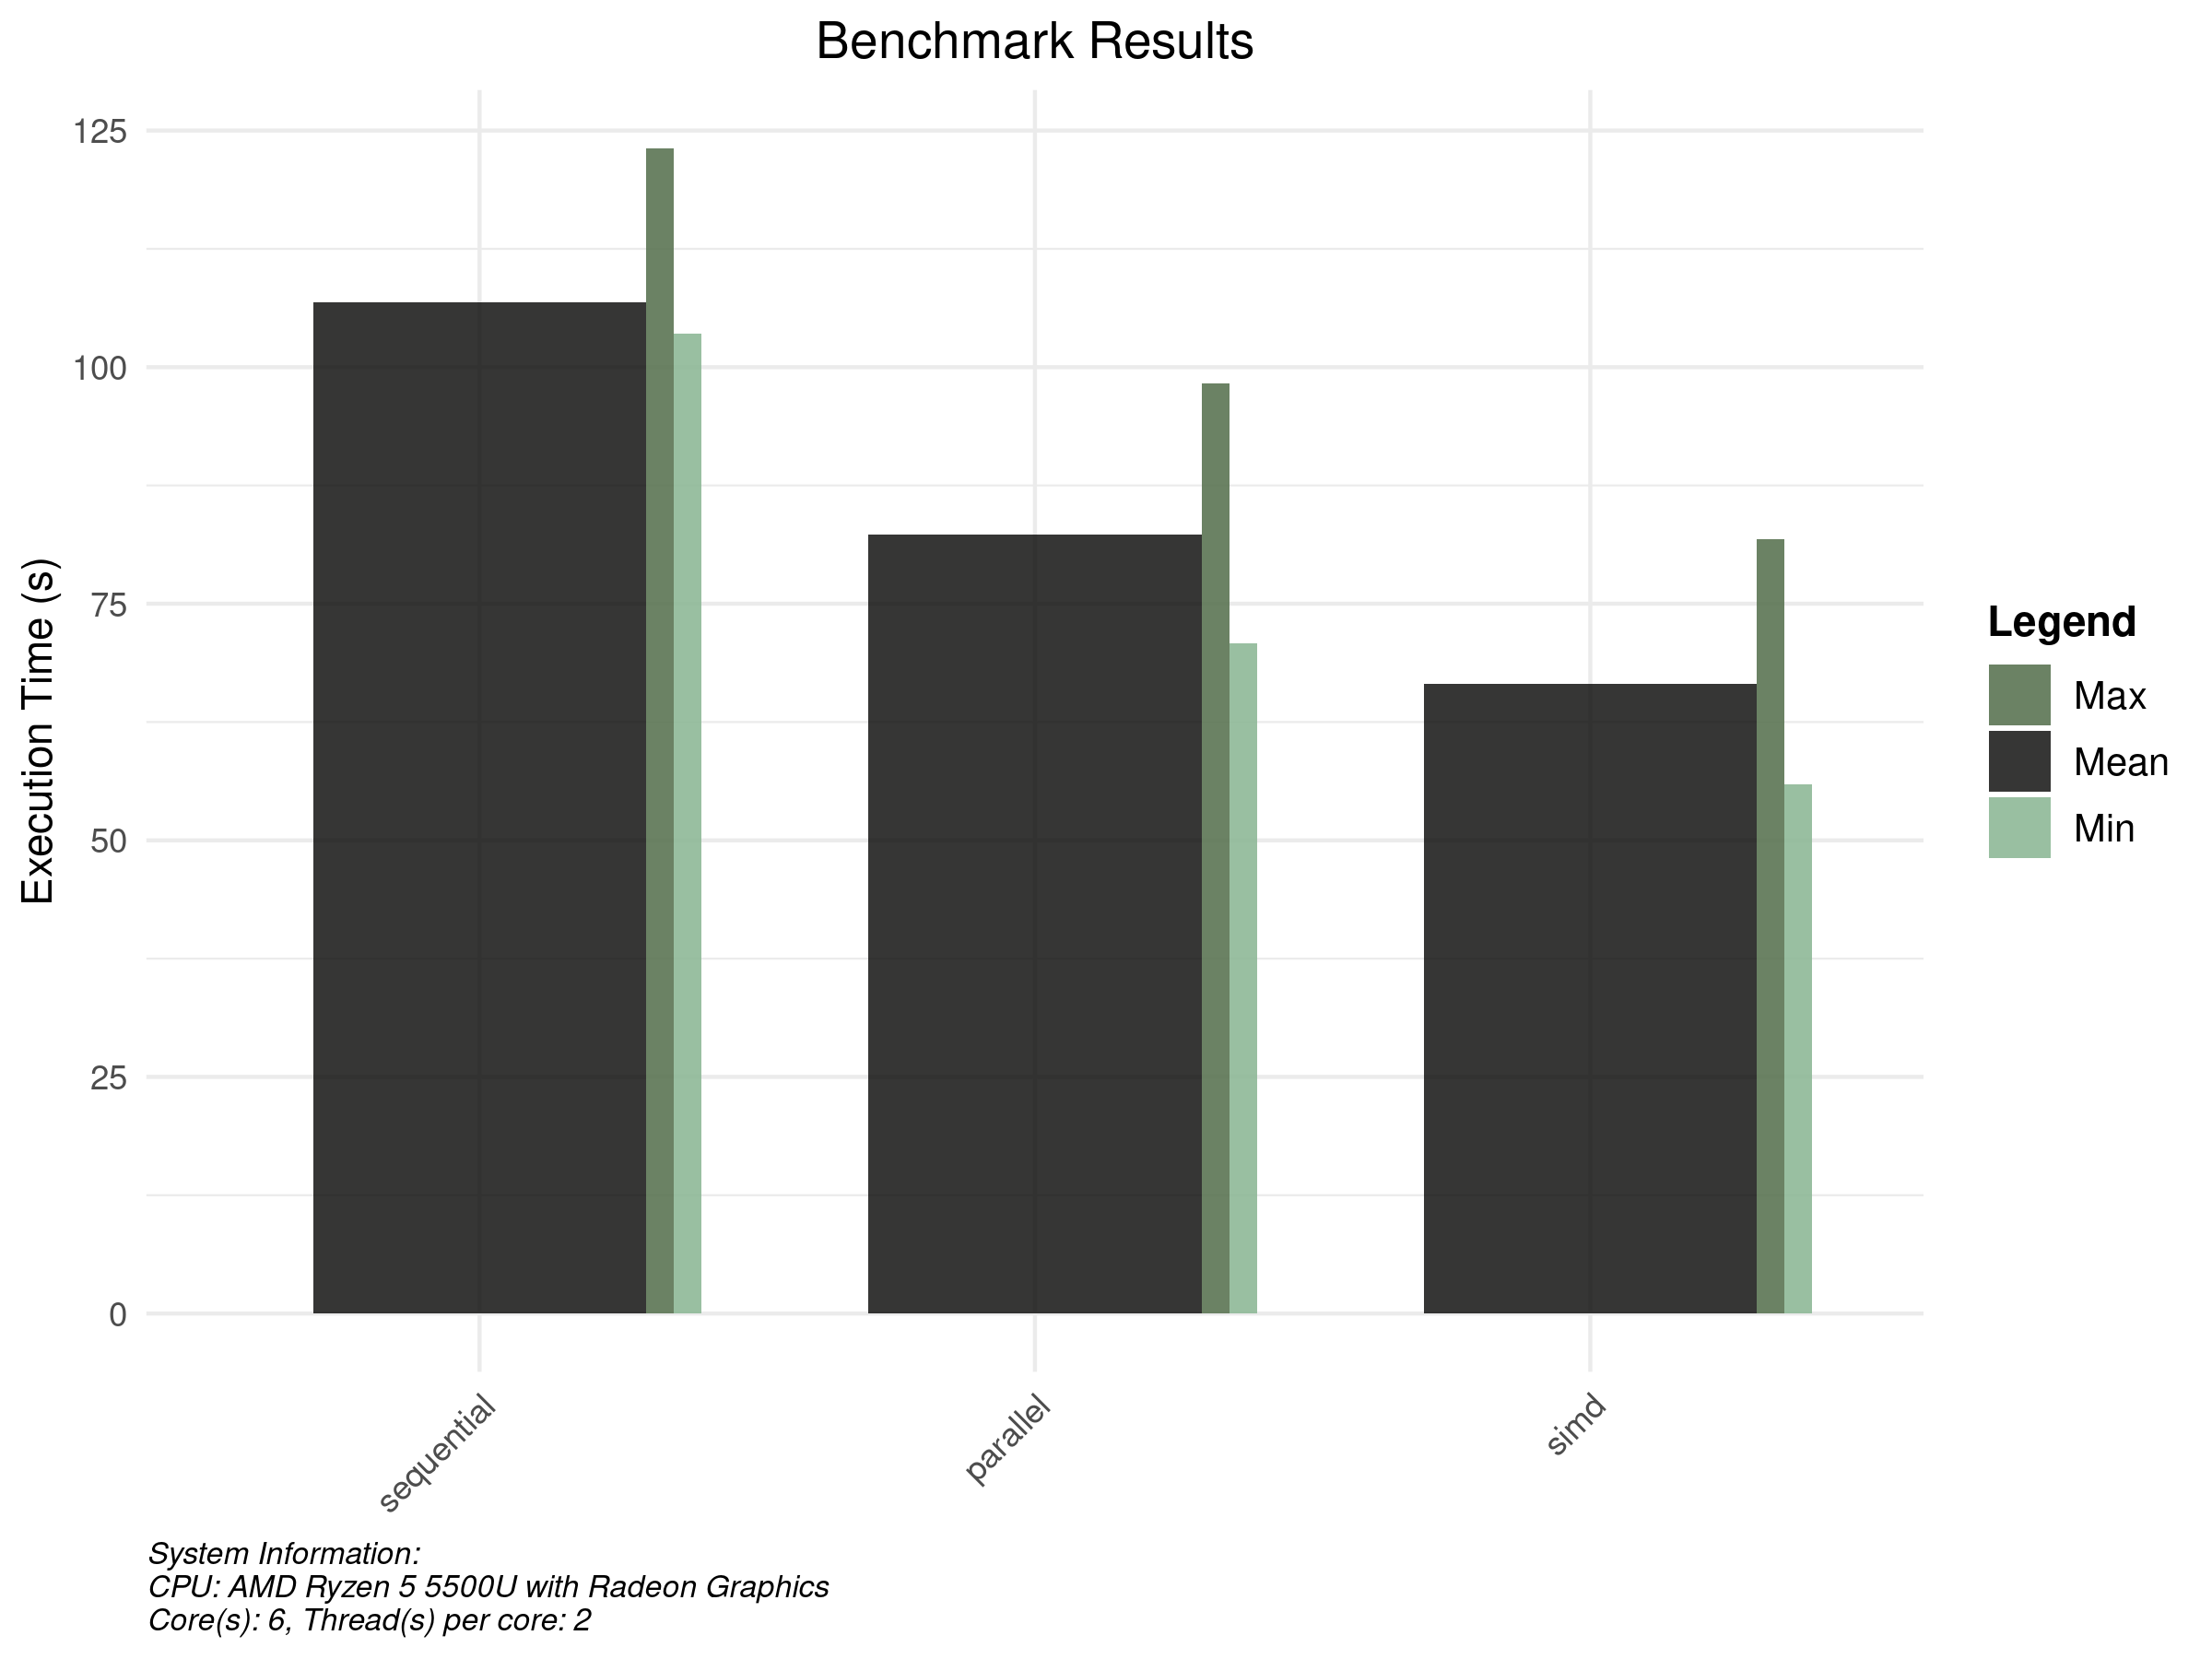
\includegraphics[width=12.5cm]{Bilders/benchmark_plot.png}
		\caption{Benchmarkergebnisse mit Hyperfine}
		\label{fig:plot}
	\end{center}
\end{figure}

\subsection{Lernfortschritt und Vorhersagbarkeit}\label{chapter..4.3}

Neben der Auswertung der Benchmarks mit \textit{Hyperfine} wurde auch die Genauigkeit der 
einzelnen Algorithmen über die Epochen hinweg analysiert und dokumentiert. Anschließend konnten 
die erfassten Daten mithilfe eines separaten R-Skripts visualisiert werden. Die grafische 
Darstellung dieser Ergebnisse ist in \autoref{fig:accuracy} zu sehen. Diese Visualisierung 
ermöglicht es, den Lernfortschritt der Algorithmen sowie deren Anpassung der Gewichte im Laufe des 
Trainingsprozesses detailliert zu untersuchen.

\begin{figure}[H]
    \begin{center}
        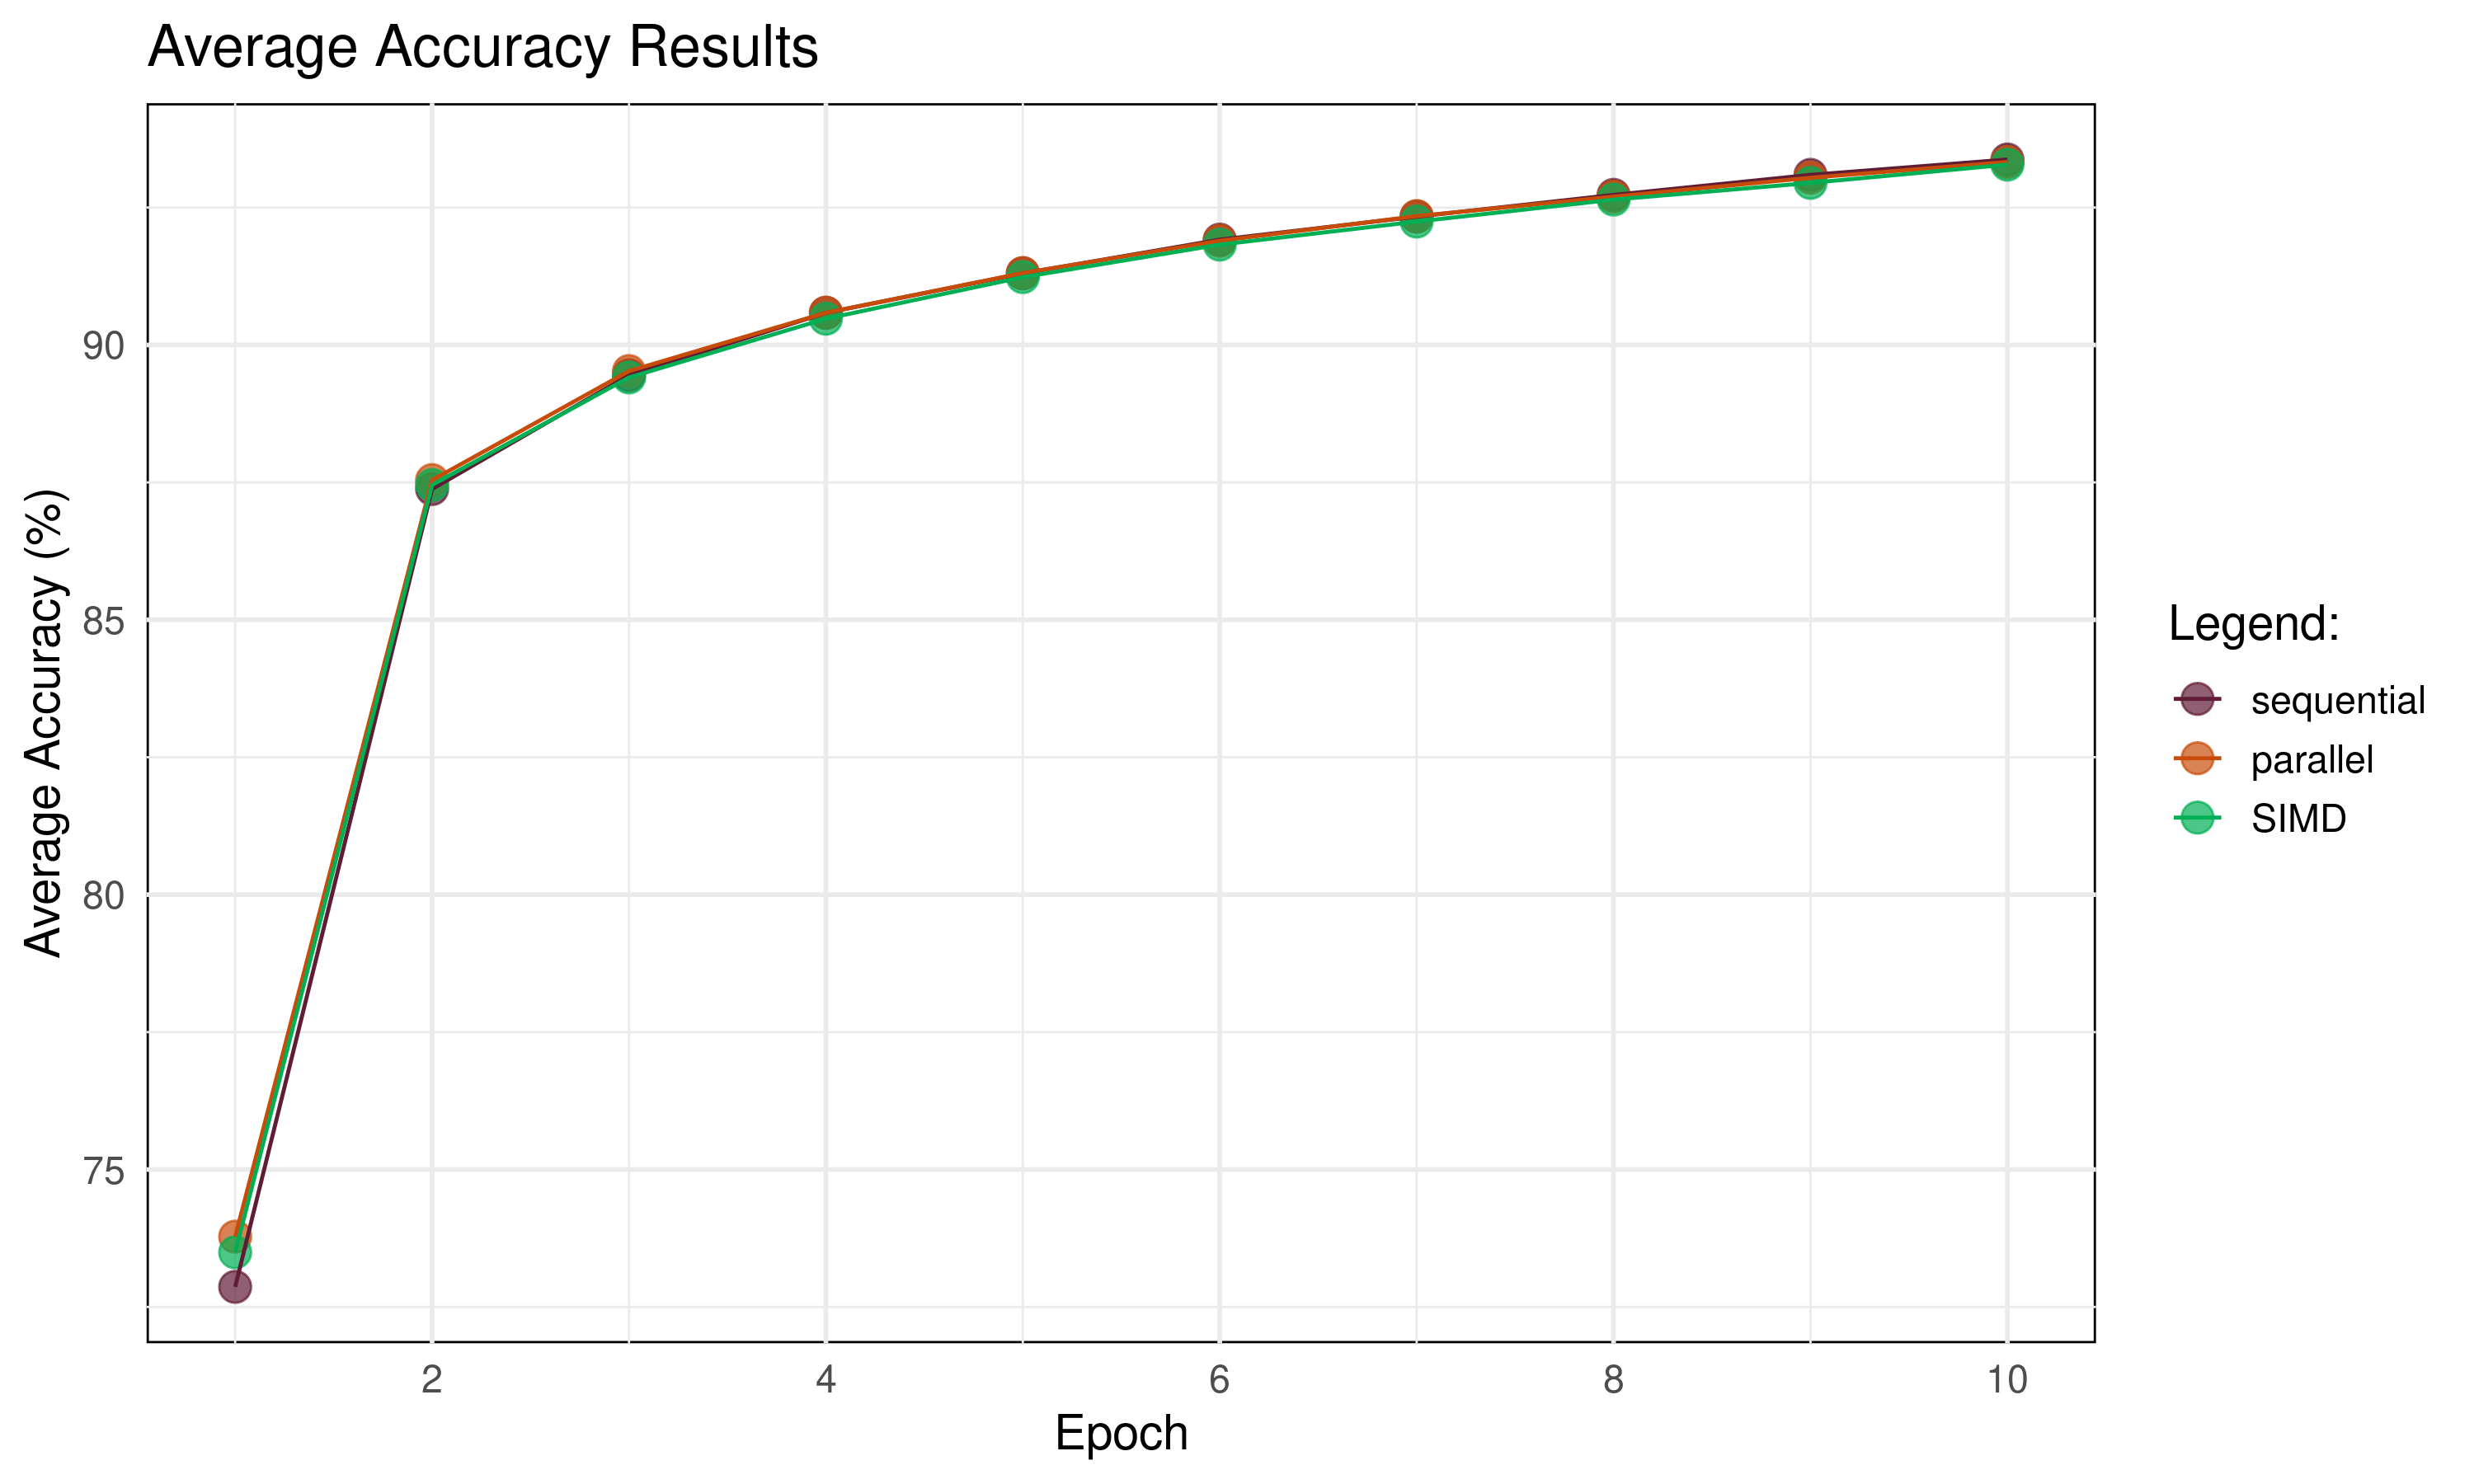
\includegraphics[width=10cm]{Bilders/accuracy_plot.png}
        \caption{Mittelwerte der Genauigkeiten}
        \label{fig:accuracy}
    \end{center}
\end{figure}

Zu sehen ist die Genauigkeit der einzelnen Algorithmen über den zeitlichen Verlauf der Epochen 
ihrer Trainingsphasen. Während der Trainingsphase wurden für jeden Algorithmus zehn unabhängige 
Testzyklen durchlaufen. Anschließend wurden die Ergebnisse gemittelt, um potenzielle Ausreißer 
zu minimieren. \autoref{fig:accuracy2} hingegen zeigt die absoluten Messergebnisse, 
ohne mathematische Glättung.

\begin{figure}[H]
    \begin{center}
        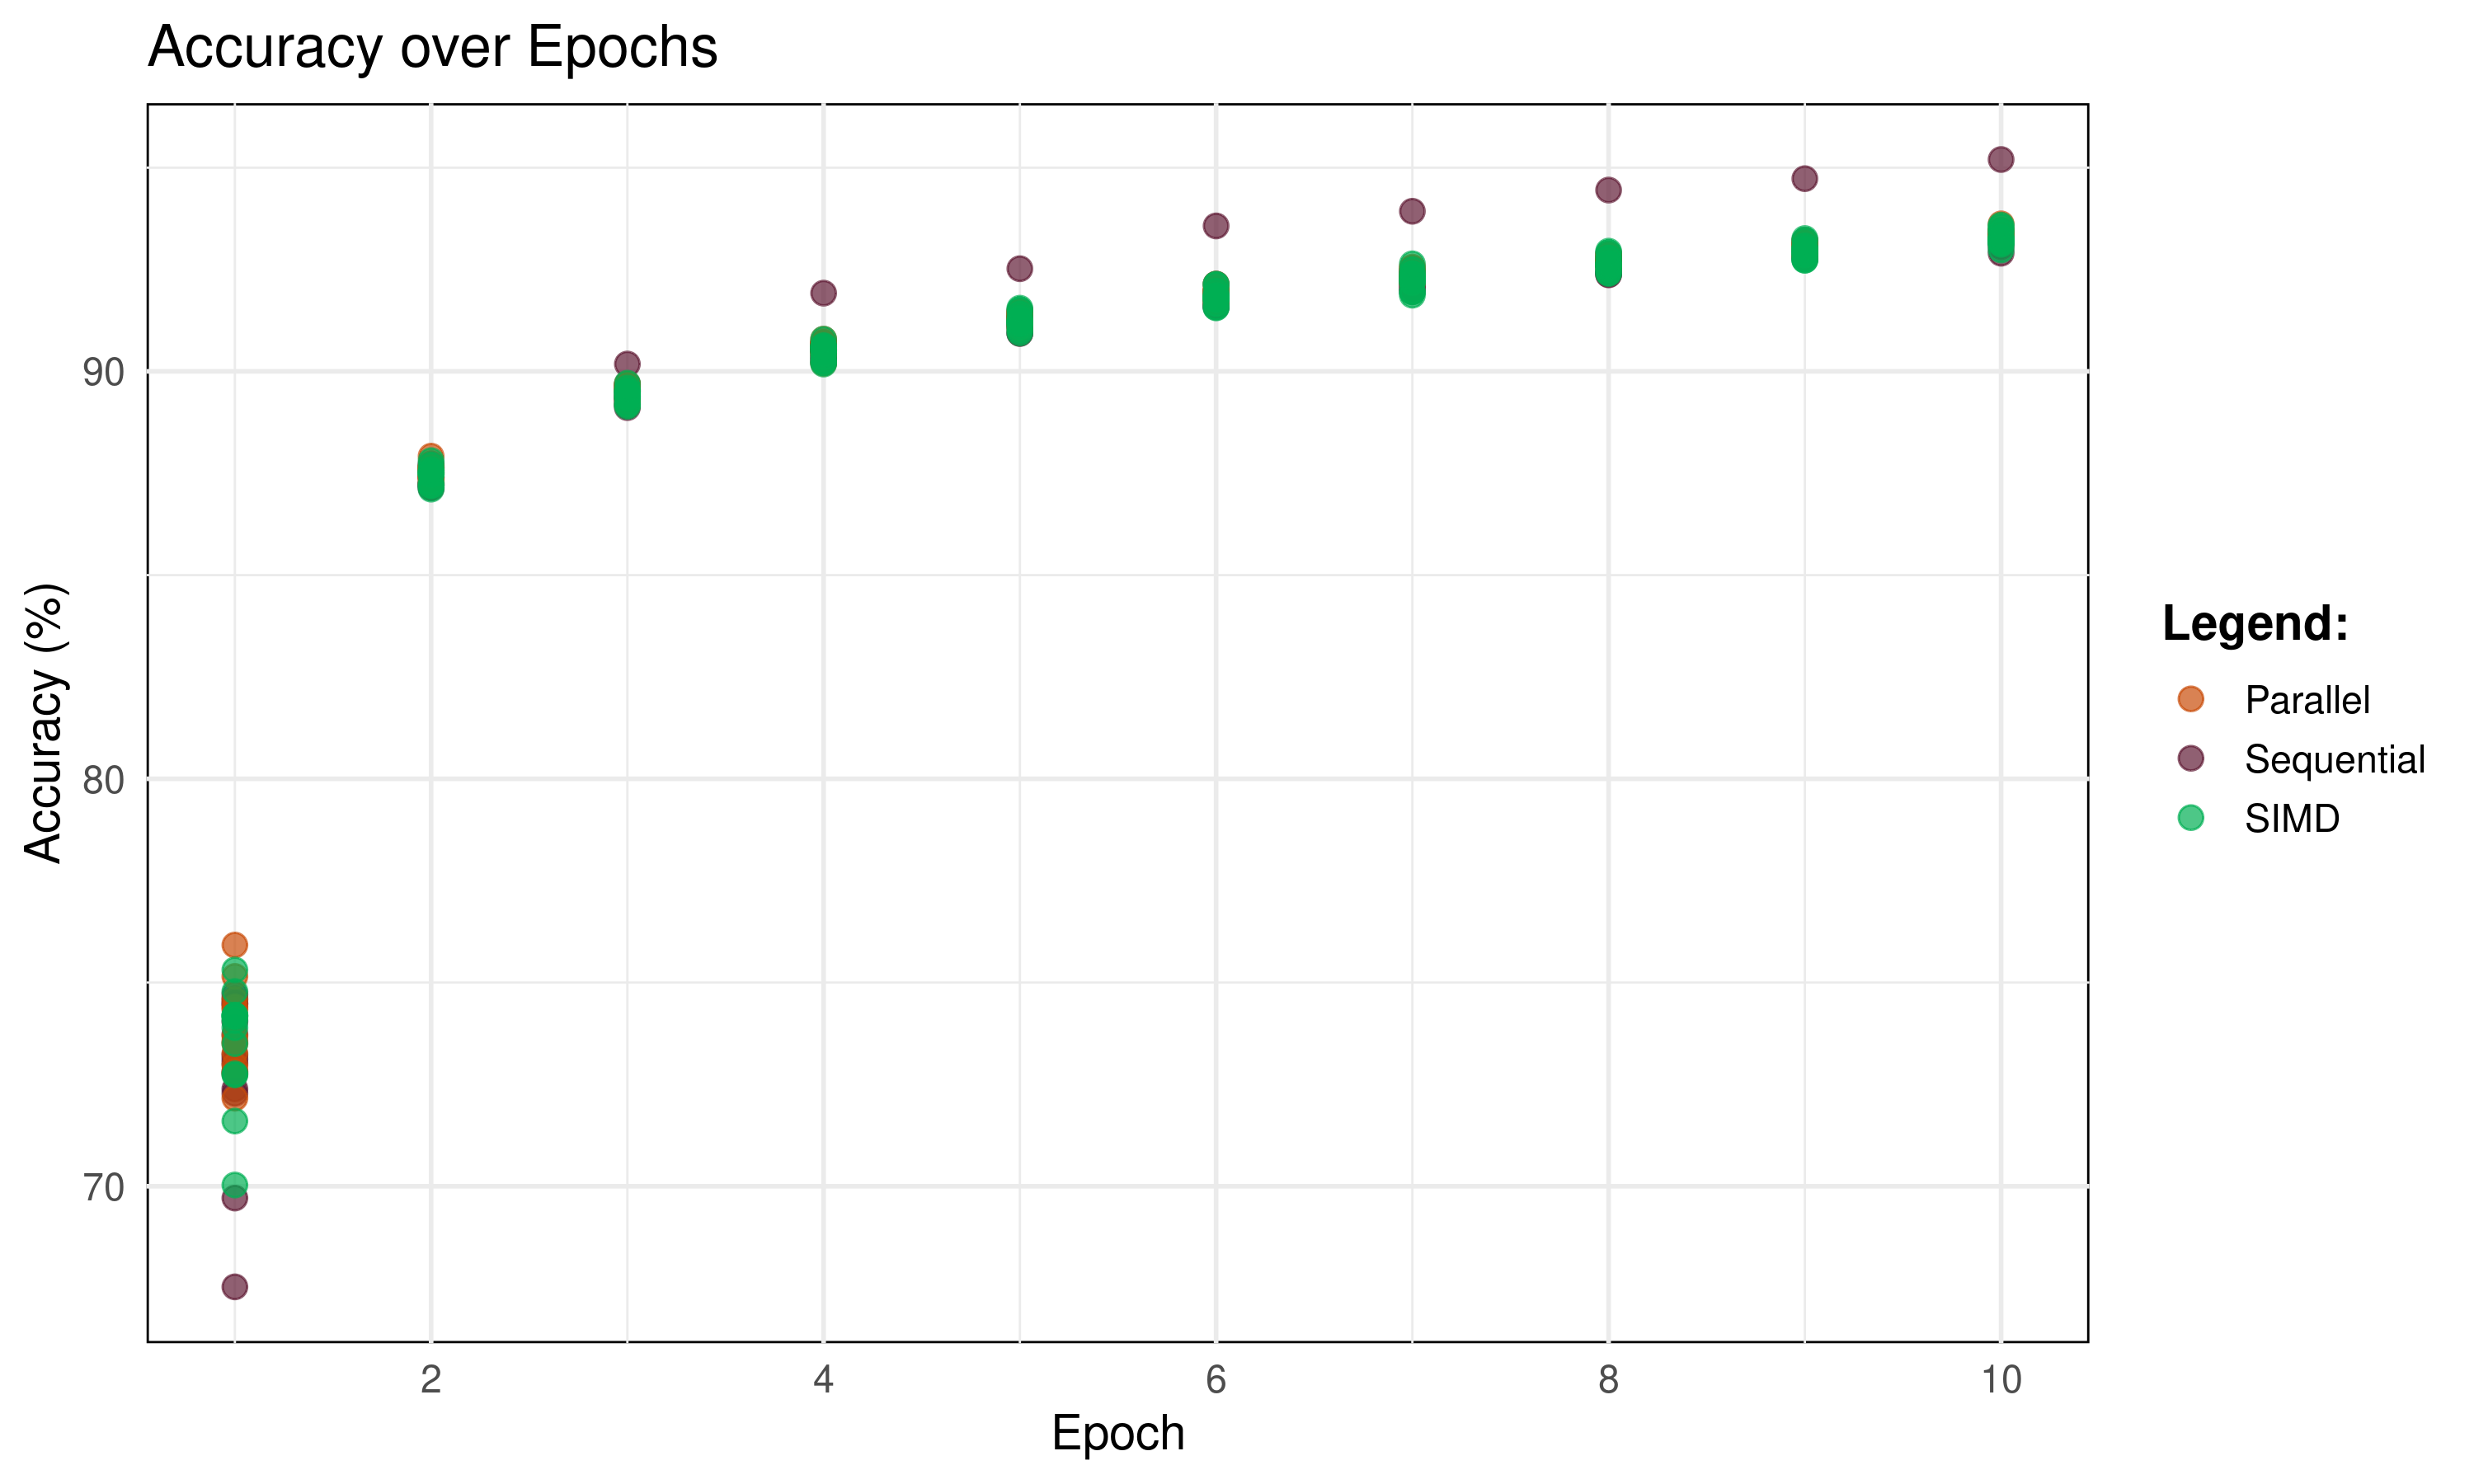
\includegraphics[width=10cm]{Bilders/accuracy_plot2.png}
        \caption{Genauigkeiten der einzelnen Algorithmen}
        \label{fig:accuracy2}
    \end{center}
\end{figure}


\newpage %PAGEBREAK
\clearpage

\section{Auswertung und Fazit}

\newpage %PAGEBREAK

\bibliographystyle{plain}
\bibliography{refs}

\end{document}
